
En traitement du signal, la phase d'un signal est intrinsèquement liée à la notion de fréquence instantanée, qui joue un rôle important en analyse temps-fréquence. 
C'est donc de ce point que commencera notre discussion pour introduire la phase géométrique.
Pour cela, seront rapidement introduites quelques notions et résultats d'analyse temps-fréquence dans le cas univarié (sec. \ref{subsec:ana_temp-freq}). Suite à quoi, une notion de phase instantanée sera proposée dans le cas multivarié (sec. \ref{subsec:intro_phased}), ce qui permettre, enfin, de mettre en évidence la phase géométrique (sec. \ref{subsec:intro_phaseg}).
\\

Dans une seconde partie, seront introduits les signaux bivariés dits AM-FM-PM, dont la phase géométrique sera calculée explicitement (sec. \ref{subsec:AM-FM-PM}), ce qui permettra de mettre en évidence certaines de ses propriétés (sec. \ref{subsec:phase_g2Poincare}). Dans une dernière section, seront proposées des généralisations des signaux AM-FM-PM au delà du cas bivarié (sec. \ref{subsec:aller_plus_loin}), ce qui mènera au formalisme de la \cref{part:phase_geo} suivante.
\\




\section{Introduction de la phase géométrique} \label{sec:intro_phaseg}

\subsection{Cas univarié : signaux AM-FM} \label{subsec:ana_temp-freq}


En traitement du signal, l'analyse fréquentielle par la transformée de Fourier est un incontournable. 
Seulement, cette transformation fait perdre toute notion temporelle : si l'étude du spectre du signal permet de dire quelles fréquences apparaissent dans le signal, elle ne permet pas de dire à quel(s) moment(s). 
C'est en réponse à cela, entre autre, que fut développée l'analyse temps-fréquence et, à cette fin, sont définis les paramètres instantanées d'un signal :\par

\begin{definition}[Paramètres instantanés] \label{def:param_instant}
	Soit $x$, est un signal complexe écrit sous forme exponentielle :
	\begin{align}
		x\ &:\ \begin{aligned}\R\ &\lr\qquad \C \\
			t\ &\longmapsto\ a(t)e^{i\phi(t)}
		\end{aligned}  &  \text{où }\quad a(t)\in\R^+\quad &\text{et}\quad \phi(t)\in\R
	\end{align}
	$a$ est appelé \emph{amplitude instantanée} du signal, $\nicefrac{1}{2\pi}\phi'$ sa \emph{fréquence instantanée} et sa \emph{phase instantanée} est définie --- modulo un choix de phase initiale --- par :
	\begin{equation} \label{eq:phasei}
		\phasei(x,t_0,t) = \phi(t) - \phi(t_0)
	\end{equation}
\end{definition}
\skipl 

Pour les signaux réels, ces notions sont moins évidentes à définir puisqu'elles demandent d'écrire les signaux sous la forme :
\[x(t) = a(t) \cos\phi(t)\]
\\
Auquel cas, le choix de la pair $(a,\phi)$ n'est pas unique. Il existe tout de même un ``bon'' choix dans le cas des signaux AM-FM :
\begin{definition}[Signal AM-FM]
	Un signal réel de la forme :
	\begin{align}
		x\ &:\ \begin{aligned}\R\ &\lr\qquad \R \\
			t\ &\longmapsto\ a(t) \cos\phi(t)
		\end{aligned}  &  \text{où }\quad a(t)\in\R^+\quad
	\end{align}
	est dit \emph{AM-FM} (\emph{amplitude and frequency modulated}) si $a$ et $\cos\phi$ admettent des transformée de Fourier et si, de plus, la première a un spectre concentré sur les bases fréquences, la seconde concentré sur les hautes fréquences et que les deux ne se chevauche pas.
	Formellement, ces conditions demande qu'il existe $\lambda\in\R^+$ telle que :
	\begin{equation}\label{eq:condi_AM-FM}
		\supp \Fou{a} \subset [-\lambda, \lambda],\quad \supp \Fou{\cos\phi} \subset \R\setminus[-\lambda,\lambda]
	\end{equation}
	\\
	Dans ce cas, $a$ et $\phi$ donne lieu au même vocabulaire que pour le cas complexe (\cref{def:param_instant}).
\end{definition}
\skipl
\\
Ces conditions sont liées au théorème de Bedrosian, et plus de détails se trouvent dans l'annexe \ref{ann:complement_t-f}. Pour le dire rapidement, exiger que toutes les hautes fréquences de $x$ se trouvent dans la phase traduit l'idée que l'amplitude doit moduler la phase, et non l'inverse. Une autre façon de le dire est que cela évite que toutes les fréquences puissent se trouver dans l'amplitude $a$, auquel cas, $x$ n'aurait ``pas de fréquence'' au sens où $\phi$ pourrait être choisie constante, voir nulle.
\\
Sous ces conditions, $x$ peut être vu comme le signal complexe $\SA{x}$ telle que :
\begin{equation}
	\forall t\in\R,\qquad \SA{x}(t) = a(t) e^{i\phi(t)}= a(t)\cos\phi(t) + ia(t)\sin\phi(t)
\end{equation}
\\
Ce signal $\SA{x}$ est appelé \emph{transformée en signal analytique de} $x$ et a, par construction, les mêmes paramètres instantanée que $x$.
Là encore, le lecteur est renvoyé vers l'annexe \ref{ann:complement_t-f} pour plus de détails ou bien dans le livre de Cohen \cite{cohen_time_1995}.
\\

L'intérêt d'introduire toutes ces notions est que les signaux multivariés --- même complexe --- souffrent du même problème que les signaux réels. 
En effet, en écrivant un signal $\x$ sous la forme :
\[\forall t\in\R,\qquad 
\x(t) = \begin{pmatrix} A_1(t)e^{i\phi_1(t)} \\ A_2(t)e^{i\phi_2(t)} \\ \vdots \\ A_n(t)e^{i\phi_n(t)}
\end{pmatrix}\]
\\
le fait que $\x$ soit à valeur dans $\C^n$ impose un choix naturel d'amplitude instantanée : sa norme. Pour ce qui est de la phase instantanée, en revanche, n'importe qu'elle choix de $\phi$ convient \apriori. En écrivant :
\[\forall t\in\R,\qquad 
\x(t) = \begin{pmatrix} A_1(t)e^{i\phi_1(t)} \\ A_2(t)e^{i\phi_2(t)} \\ \vdots \\ A_n(t)e^{i\phi_n(t)} \end{pmatrix}
= a(t)e^{i\phi(t)}\begin{pmatrix} a_1(t)e^{i\psi_1(t)} \\ a_2(t)e^{i\psi_2(t)} \\ \vdots \\ a_n(t)e^{i\psi_n(t)} \end{pmatrix}
\qquad\text{ avec }\qquad 
\left\{ \begin{aligned}
	& a(t) = \| \x(t) \|_2 \\
	& \big\|(a_i)_{1\leq i\leq n}\big\|_2 = 1 \\
	& \phi_i = \phi + \psi_i \end{aligned}\right.\]
\\
il suffit que les $\psi_i$ soient ajustés pour assurer que $\ \phi_i = \phi + \psi_i$.
\\
\begin{remarque}
	Si $a$ et $\phi$ correspondent respectivement à une amplitude et une phase, le vecteur restant $\big( a_ie^{\phi_i} \big)_{1\leq i\leq n}$ correspond à un état de polarisation, sur lequel nous reviendrons dans la \cref{sec:AM-FM-PM} suivante.
\end{remarque}
\skipl




\subsection{Phase et fréquence instantanée de signal multivarié }\label{subsec:intro_phased}

On se propose ici de définir la phase instantanée comme suit :
\begin{definition}[Phase dynamique/instantanée] \label{def:phase_d}
	La \emph{phase instantanée} ou \emph{dynamique} (à l'instant $t$ partant de $t_0$) d'un signal multivarié $\x = a\big(a_ie^{i\phi_i}\big)_{1\leq i\leq n} \in \conti[1]{\R}{\C^n}$, est donnée par la formule :
	\begin{equation} \label{eq:phase_d}
		\forall t_0, t\in\R, \quad \phased(\x, t_0,t) \defeq \int_{t_0}^t \frac{\Im m \big\langle \dot{\x}(s) , \x(s) \big\rangle}{\|\x(s)\|^2} ds =\sum_{i=1}^n \int_{t_0}^t a_i(s)^2 \phi_i'(s)ds
	\end{equation}
	\\
	L'on s'autorisera à omettre les paramètres de $\phased$ lorsque cela ne prête pas à confusion.
\end{definition}
\skipl

Cette définition est motivée par deux arguments :



\subsubsection*{Argument variationnel}

Le premier, fortement inspiré par les travaux de Lilly \& Olhede  \cite{lilly_analysis_2012}, consiste à généraliser la condition \eqref{eq:condi_AM-FM} de séparation haute/basse fréquences sur les signaux AM-FM.
Pour cela, l'on commence par faire apparaître une phase $\phi$ --- pour l'instant inconnue --- en écrivant $\x$ sous la forme :
\[\forall t\in\R,\qquad \x(t) = e^{i\phi(t)} e^{-i\phi(t)} \x(t) \defeq e^{i\phi(t)} \bf{y}(t)\]
\\
Si $\phi$ est bien choisie, alors $\bf{y}$ ne devrait contenir que les informations associées à l'amplitude et à la polarisation de $\x$. Or, conformément à la condition \eqref{eq:condi_AM-FM}, la phase doit contenir les hautes fréquences du signal et, inversement, les basses fréquences doivent se trouver dans le reste. 
\\
La fréquence donnant, pour le dire vite, la vitesse d'ondulation, la contrainte sur $\x$ va être de limite les variations de  $\bf{y}$. Concrètement, $\phi$ doit être choisie de sorte à minimiser la dérivée $\dot{\bf{y}}$ :
\[\forall t\in\R,\qquad \phi(t) = \argmin{\theta(t)}{\big\|\dot{\bf{y}}(t)\big\|_2}^2 = \argmin{\theta(t)}{\Big\|e^{-i\theta(t)}\big(\dot{\x}(t) - i\theta'(t) \x(t)\big) \Big\|_2}^2 = \argmin{\theta(t)}{\big\|\dot{\x}(t) - i\theta'(t)\x(t)\big\|_2}^2\]
\\
La contrainte ne dépendant que de la dérivée $\theta'$, on se ramène à :
\[\min_{\theta(t)}{\|\dot{\bf{y}}(t)\|_2}^2 = \min_{\theta'(t)}{\big\|\dot{\x}(t) - \theta'(t) \x(t)\big\|_2}^2\]
\\
En rappelant que $\frac{d}{dx}{\big\|f(x)\big\|_2}^2 = 2\Re e\big\langle f(x), f'(x)\big\rangle$, il vient que ce minimum\footnote{\itshape
	L'extremum obtenu est l'unique minimum globale puisque $t\longmapsto \|at + b\|^2$ est strictement convexe pour $a\neq0$.}
est atteint par $\phi'(t)$ à condition que :
\begin{align*}
	\frac{d}{d\phi'}{\big\| \dot{\x} - i\phi' \x\big\|_2}^2 = 0 \quad \Llr\quad
	0 &= 2\Re e\left\langle  \dot{\x} - i\phi' \x ,  \frac{d}{d\phi'}\big(\dot{\x} - i\phi' \x\big)\right\rangle \\
	&= 2\Re e\big\langle  \dot{\x} - i\phi' \x ,  - i \x\big\rangle \\
	&= 2\Re e\Big(i\big\langle  \dot{\x} ,  \x\big\rangle\Big) + 2\phi'\Re e\big\langle   \x ,  \x\big\rangle\\
	&= -2\Im m\big\langle  \dot{\x} ,  \x\big\rangle + 2\phi'{\| \x\|_2}^2
\end{align*}
Ainsi $\displaystyle \ \phi' = \frac{\Im m\big\langle  \dot{\x} ,  \x\big\rangle}{{\| \x\|_2}^2}\ $ et :
\begin{equation}\label{eq:phas_inst_v1}
  \phi(t) = \Im m\int_{t_0}^t \frac{\big\langle \dot{\x}(s) , \x(s) \big\rangle}{\|\x(s)\|^2} ds = \phased(\x,t_0,t)
\end{equation}
\skipl




\subsubsection*{Arguments des moyennes}

Le second argument, cette fois inspiré de \cite{cano_mathematical_2022}, se base sur la notion de fréquence moyenne.
D'abord dans le cas d'un signal complexe univarié, sont définies les fonctions de densités d'énergie (resp. d'énergie spectrale) comme :
\begin{align}\label{eq:densi_dE}
	\densit\ &:\quad \begin{aligned}\R\ &\lr\quad \R^+ \\ t\ &\longmapsto\ \big|x(t)\big|^2 \end{aligned}  
	&
	\text{resp.}\qquad \densis\ &:\quad \begin{aligned}\R\ &\lr\quad \R^+ \\ \nu\ &\longmapsto\ \big|\fou{x}(\nu)\big|^2 \end{aligned}
\end{align}
\\
À partir de ces dernières est définie la fréquence moyenne de $x$ comme comme l'espérance $\esp[\densis]{\nu}$ de $\densis$. Cette fréquence moyenne est liée à la fréquence instantanée par la formule\footnote{\itshape
	Cette formule de généralise à tout les moments de $\densis$ et existe également pour les moments de $\densit$, voir \cite[sec. 1.4]{cohen_time_1995} pour une démonstration ``à la physicienne''
} :
\begin{equation}\label{eq:esp_freq}
	\esp[\densis]{\nu} = \frac{1}{2\pi}\int_\R \phi'(t)\densit(t)dt = \frac{1}{2\pi} \esp[\densit]{\phi'}
\end{equation}
\\
Dans le cas d'un signal $\x=(x_i)_{1\leq i\leq n}$ multivarié, les densités d'énergies se définissent comme :
\begin{align*}%\label{eq:densi_dEi}
	\densit_i\ &:\quad \begin{aligned}\R\ &\lr\quad \R^+ \\ t\ &\longmapsto\ \big|x_i(t)\big|^2 = a(t)^2 a_i(t)^2 \end{aligned}  
	&
	\densis_i\ &:\quad \begin{aligned}\R\ &\lr\quad \R^+ \\ \nu\ &\longmapsto\ \big|\fou{x}_i(\nu)\big|^2 \end{aligned} \\ \\
	%\label{eq:densi_dE-mv}
	\densit\ &:\quad \begin{aligned}\R\ &\lr\quad \R^+ \\ t\ &\longmapsto\ \big\|\x(t)\big\|^2 = \sum_{i=1}^n \densit_i(t) \end{aligned}  
	&
	\densis\ &:\quad \begin{aligned}\R\ &\lr\quad \R^+ \\ \nu\ &\longmapsto\ \big\|\fou{\x}(\nu)\big\|^2 = \sum_{i=1}^n \densis_i(t) \end{aligned}	
\end{align*}
Le second argument consiste alors à dire que l'égalité des moyennes $\eqref{eq:esp_freq}$ doit rester valable dans le cas multivarié. Cela assure, a minima, que la fréquence instantanée de $\x$, $\nicefrac{1}{2\pi}\phi'$, à pour moyenne $\esp[\densis]{\nu}$.
\\

En appliquant la formule \eqref{eq:esp_freq} au $\densis_i$, et en notant toujours $\x = a\big(a_ie^{i\phi_i}\big)_{1\leq i\leq n}$, on obtient :
\begin{align*}
	\esp[\densis]{\nu} = \int_\R \nu\densis(\nu)d\nu &= \int_\R \nu\sum_{i=1}^n \densis_i(\nu) d\nu \\
	&= \sum_{i=1}^n\esp[\densis_i]{\nu} \\
	&= \sum_{i=1}^n\frac{1}{2\pi}\int_\R \phi_i'(t)\densit_i(t)dt \\
	&= \frac{1}{2\pi}\int_\R a(t)^2\sum_{i=1}^n\phi_i'(t)a_i(t)^2 dt 
	\\ &= \frac{1}{2\pi} \esp[\densit]{\sum_{i=1}^n \phi_i'{a_i}^2}
\end{align*}
\\
Ce qui mène à poser $\displaystyle \ \sum_{i=1}^n \phi_i'(t){a_i}^2(t)\ $ pour la fréquence instantanée, avec la phase associée :
\begin{equation}\label{eq:phas_inst_v2}
	\phi = \int_{t_0}^t \sum_{i=1}^n \phi_i'(s){a_i}(s)^2ds 
	= \sum_{i=1}^n \int_{t_0}^t \phi_i'(s){a_i}(s)^2ds 
	%= \sum_{i=1}^n \esp[\nicefrac{\densit_i}{\densit}]{\phi_i'}
\end{equation}
\\

Formule qui concorde bien avec celle de la phase dynamique une fois explicitée :
\begin{align*}
	\Im m\frac{\big\langle \dot{\x}(t) , \x(t) \big\rangle}{\|\x(t)\|^2} &= \Im m\left( \frac{1}{a(t)^2} \sum_{i=1}^n \Big( \big(aa_i\big)'(t) +a(t)a_i(t)i\phi_i'(t)\Big)e^{i\phi_i(t)}\congu{a(t)a_i(t)e^{i\phi_i(t)}} \right) \\
	&=\frac{1}{a(t)^2}  \Im m\left( \sum_{i=1}^n a(t)a_i(t)\big(aa_i\big)'(t) +ia(t)^2a_i(t)^2\phi_i'(t) \right) \\
	&= \frac{1}{a(t)^2} \sum_{i=1}^n a(t)^2a_i(t)^2 \phi_i'(t) \\
	&= \sum_{i=1}^n a_i(t)^2 \phi_i'(t)
\end{align*}
D'où
\[\Im m\int_{t_0}^t \frac{\big\langle \dot{\x}(s) , \x(s) \big\rangle}{\|\x(s)\|^2} ds = \int_{t_0}^t \sum_{i=1}^n a_i(s)^2 \phi_i'(s) = \sum_{i=1}^n \int_{t_0}^t a_i(s)^2 \phi_i'(s)ds\]
\skipl



\subsection{Apparition de la phase géométrique}\label{subsec:intro_phaseg}

Cela étant dit, il existe une autre façon, plus simple, d'obtenir la phase d'un signal. D'abord, dans le cas univarié, la phase instantanée de $x=ae^{i\phi}$ peut être réécrite comme :
\[\phi(t)-\phi(t_0)  = \arg\left( x(t) \congu{x(t_0)} \right)\]
\\
Formule qui se généralise en cas multivarié par ce qui sera appelé la \emph{phase totale} du signal :
\begin{equation}\label{eq:phase_t}
	\phaset(\x, t_0, t) \defeq \arg\big\langle \x(t), \x(t_0)\big\rangle
\end{equation}
\\
D'un point de vu géométrique, il est bien connue que le produit scalaire entre deux vecteurs réels $u,v\in\R^n$ est lié à l'angle $\angle(u,v)$ entre ces derniers par la formule :
\[\langle u,v\rangle_\R = \|u\|^2 \|v\|^2 \cos \angle(v,u)\]
\\
Pour le produit hermitien, cet angle ce retrouve dans l'argument, de sorte que si $u$ et $v$ sont complexes :
\[\langle u,v\rangle_\C = \|u\|^2 \|v\|^2 e^{i \angle(v,u)}\]
\\
En ce sens, la phase totale calcule explicitement l'angle entre $\x(t_0)$ et $\x(t)$ et il est montré, dans le cas en univarié, qu'elle est égale à la phase dynamique. En effet, pour $\x = ae^{i\phi}$ :
\begin{align*}
	\phased(\x) = \Im m\int_{t_0}^t \frac{\big\langle \dot{\x}(s) , \x(s) \big\rangle}{\|\x(s)\|^2} ds &= \Im m \int_{t_0}^t \frac{\big(a'(s) + ia(s)\phi'(s) \big) e^{i\phi(s)} \congu{a(s) e^{i\phi(s)}}}{a^2(s)} ds \\
	&= \int_{t_0}^t \frac{a^2(s)\phi'(s))}{a^2(s)} ds \\
	&= \phi(t) - \phi(t_0) = \phaset(\x)
\end{align*}
\skipl

Dans le cas multivarié, en revanche, c'est une autre histoire. En notant cette fois le signal $\ \x = ae^{i\phased} \big( a_ie^{\psi_i} \big)_{1\leq i\leq n}$, la phase totale se réécrit :
\begin{equation}\label{eq:diff_phases_t/d}
	\begin{aligned}
		\phaset(\x,t_0, t) &= \arg \left(a(t)a(t_0) e^{i\big(\phased(t) - \phased(t_0)\big)}\sum_{i=1}^n a_i(t)a_i(t_0)e^{i(\psi_i(t)-\psi_i(t_0))} \right) \\
		&= \phased(t) + \arg \left(\sum_{i=1}^n a_i(t)a_i(t_0)e^{i(\psi_i(t)-\psi_i(t_0))} \right)  \qquad\qquad\qquad\qquad \text{car } \phased(t_0,t_0) = 0
		%\\ &= \phased + \arctan \left( \frac{\sum_i a_i(t)a_i(t_0)\sin\big( \psi_i(t)-\psi_i(t_0)\big)}{\sum_i a_i(t)a_i(t_0)\cos\big( \psi_i(t)-\psi_i(t_0)\big)}  \right)
	\end{aligned}
\end{equation}
\\
Apparaît alors un terme de déviation de la phase dynamique par rapport à la phase totale, appelé (surprise) phase géomatique et noté :
\begin{equation}\label{eq:phase_g}
	\phaseg(\x,t_0,t) \defeq \phaset(\x, t_0,t) - \phased(\x, t_0,t)
\end{equation}
Cette déviation s'observe expérimentalement, comme le montre la \Cref{fig:calc_diff_phases} ci-dessous.
\\
\begin{figure}[h]
	
\includegraphics[width=0.6\textwidth]{fig/placeholder}
	\caption[Déviation de la phase dynamique par rapport à la phase totale]{Sur le graphe de gauche, le signal $\x$ est à valeurs dans $\R^2$ et dans celui de droite le calcul des phases dynamique et totale ainsi que de leur différence. %Résultat tiré des simulation de Le Bihan \etal~\cite{le_bihan_modephysiques_2023}
	}
	\label{fig:calc_diff_phases}
\end{figure}
\\

Comme mentionné en introduction, un résultat bien connu en physique \cite{bohm_geometric_2003,mukunda_quantum_1993,chruscinski_geometric_2004} est que cette troisième phase est invariante par transformation de jauge et par reparamétrisation.
Dans notre contexte, cela signifie d'une part que si $\x$ et $\Tilde{\x}$ sont deux signaux multivariés complexes tels que $\ \Tilde{\x} = e^{i\alpha}\x$, avec $\alpha$ une \underline{fonction} dérivable du temps, alors :
\begin{align*}
	\phaseg(\Tilde{\x}) &= \phaset(\Tilde{\x}) - \phased(\Tilde{\x})  = \phaset(\x) - \phased(\x) = \phaseg(\x)\\
	%&= \arg\big\langle \Tilde{\x}(t), \Tilde{\x}(t_0)\big\rangle - \Im m\int_{t_0}^t \frac{\big\langle \dot{\Tilde{\x}}(s) , \Tilde{\x}(s) \big\rangle}{\|\Tilde{\x}(s)\|^2} ds \\
	%&= \arg\big\langle e^{i\alpha(t)}\x(t), e^{i\alpha(t_0)}\x(t_0)\big\rangle - \Im m\int_{t_0}^t \frac{\big\langle \dot{e^{i\alpha(s)}\x}(s) , e^{i\alpha(s)}\x(s) \big\rangle}{\|e^{i\alpha(s)}\x(s)\|^2} ds 
\end{align*}
Et d'autre part que, pour tout difféomorphisme $\gamma$ de $\R$ telle que :
\begin{align*}
	\x\circ\gamma(s_0)&=t_0  &  \x \circ\gamma(s) = t
\end{align*}
alors on a :
\[\phaseg(\x \circ \gamma, s_0, s) = \phaseg(\x, t_0, t)\]
\skipl


D'un point de vue signal, cette invariance par transformation de jauge indique que $\phaseg$ serait lié à une notion de polarisation du signal, chose que nous allons à présent mettre en évidence.
\\



\section{Première étude : cas des signaux AM-FM-PM} \label{sec:AM-FM-PM}

Pour une première étude de la phase géométrique du signal, Le Bihan \etal~se sont penchés sur un cas particulier de signal bivarié \cite{flamant_timefrequency_2019,le_bihan_modephysiques_2023, le_bihan_geometric_2024}. Ces signaux, AM-FM-PM, sont présentés dans une première partie avec le calcul explicite de leur phases --- totale, dynamique et géométrique. Puis, sera introduite la sphère de Poincaré, sur laquelle, $\phaseg$ pourra être interprétée.
Cela mènera à proposer un modèle pour décrire les signaux multivariés complexes (modèle très largement inspiré par ce qui à déjà été fait dans l'étude de la phase géométrique).
\\



\subsection{Définitions et calcul des phases} \label{subsec:AM-FM-PM}

Ces signaux AM-FM-PM viennent généraliser les signaux AM-FM univarié en tenant compte de l'état de polarisation permis par l'accès à une seconde dimension. 
En quelques mots, dans le cas le plus simple, un signal bivarié à valeurs réelles $s$ va décrire une ellipse en cours du temps. 
On parle de polarisation elliptique et $s$ va s'écrire :
\[s(t) = a \begin{pmatrix} \cos\theta & -\sin\theta \\ \sin\theta  &  \cos\theta \end{pmatrix} \begin{pmatrix} \cos\chi \cos\varphi(t) \\ \sin\chi \sin\varphi(t) \end{pmatrix}  \qquad \text{ où }\quad  a\in\R^+,\ \theta \in \left]-\frac{\pi}{2}, \frac{\pi}{2}\right],\ \chi \in \left[-\frac{\pi}{4}, \frac{\pi}{4}\right] \]
\\
Les paramètres $a$ et $\chi$ caractérisent respectivement la taille et l'excentricité de l'ellipse, $\theta$ son orientation dans le plan et $\varphi(t)$ précise où se trouve $s$ à l'instant $t$ sur cette ellipse. 
Le tout est représenté sur la \Cref{fig:ellipse2polar} ci-dessous :
\begin{figure}[H]
	%
\includegraphics[width=0.45\textwidth]{fig/placeholder}
	\makeatletter % fonction pour increasing width !
	\pgfkeys{/pgf/decoration/.cd,
		start color/.store in =\startcolor,
		end color/.store in   =\endcolor
	}
	
	\pgfdeclaredecoration{width and color change}{initial}{
		\state{initial}[width=0pt, next state=line, persistent precomputation={%
			\pgfmathdivide{50}{\pgfdecoratedpathlength}%
			\let\increment=\pgfmathresult%
			\def\x{0}%
		}]{}
		\state{line}[width=.5pt,   persistent postcomputation={%
			\pgfmathadd@{\x}{\increment}%
			\let\x=\pgfmathresult%
		}]{%
			\pgfsetlinewidth{\x/80*0.001pt+\pgflinewidth}%
			\pgfsetarrows{-}%
			\pgfpathmoveto{\pgfpointorigin}%
			\pgfpathlineto{\pgfqpoint{.75pt}{0pt}}%
			\pgfsetstrokecolor{\endcolor!\x!\startcolor}%
			\pgfusepath{stroke}%
		}
		\state{final}{%
			\pgfsetlinewidth{\pgflinewidth}%
			\pgfpathmoveto{\pgfpointorigin}%
			\color{\endcolor!\x!\startcolor}%
			\pgfusepath{stroke}% 
		}
	}
\makeatother


\begin{tikzpicture}[scale=1]
	%\draw[black, opacity=0.3] (-4.5,-4.5) grid (4.5,4.5);
	\draw[opacity=1, -Stealth] (0,-4) -- (0,4);
	\draw[opacity=1, -Stealth] (-4,0) -- (4,0);
	
	\coordinate (o) at (0,0);
	\coordinate (i) at (4,0);
	\coordinate (j) at (0,4);
	\coordinate (theta) at (40:4);
	
	
	%axis de l'ellipse
	\draw[thick, opacity=0.9, rotate = 40] (-4,0) -- (o) node[midway, below, rotate=40]{$a\cos\chi$} -- (4,0);
	\draw[thick, opacity=0.9, rotate = 40] (0,-3) -- (o) -- (0,3) node[midway, above, rotate=-50]{$a\sin\chi$};
	
	% paramètres
		
		%theta
	\draw[opacity=0.9, -stealth] (2, 0) arc [start angle=0, end angle =40, radius = 2] node[midway, right]{$\theta$};
		
		%chi
	\draw[opacity=0.8, -stealth, rotate = 40] (-2,0) arc [start angle=0, end angle =37, radius = 2] node[midway, above right]{$\chi$};
	
	\draw[opacity=0.8, rotate = 40] (-4,0) -- (0,3);
		
		%varphi
	\draw[color=blue, opacity=0.8, -stealth, rotate = 40] (0.75,0) arc [start angle=0, end angle =60, radius = 0.75] node[midway, above right]{$\varphi$};
	
	\draw[color=blue, opacity=0.8, rotate = 40] (o) -- (60:3.18);
	
	\fill[blue] (100:3.18) circle (0.05);
	
	% ellipse
	\draw[line width=0.5pt, rotate=40, decoration={width and color change, start color=black, end color=blue}, decorate] (60:3.18) arc [start angle=66.65, end angle =426.65, x radius = 4, y radius = 3];
	
\end{tikzpicture}
	\caption[Ellipse de polarisation d'un signal bivarié réel]{Ellipse de polarisation du signal $s$ sur laquelle sont représenter ses paramètres $a,\varphi,\theta,\chi$.}
	\label{fig:ellipse2polar}
\end{figure}
\skipl \\
En autorisant les paramètres de polarisation à varier au cours du temps et après une transformation en signal analytique, mentionnée dans la \cref{subsec:ana_temp-freq}, on obtient la définition suivante :
\\
\begin{definition}[Signal AM-FM-PM] \label{def:AM-FM-PM}
	Un signal bivarié complexe $\x$ \emph{AM-FM-PM} (\emph{amplitude, frequency and polarization modulated}) est caractérisé par quatre paramètres $a,\varphi,\theta$ et $\chi$, respectivement à valeurs dans $\R^+$, $\R$, $]-\frac{\pi}{2}, \frac{\pi}{2}]$ et $[-\frac{\pi}{4}, \frac{\pi}{4}]$, vérifiant :
	\begin{align}\label{eq:condi_AM-FM-PM}
		\big| \varphi'(t) \big| &\gg \big| \theta'(t) \big| ,\ \big| \chi'(t) \big| ,\ \left| \frac{a'(t)}{a(t)}\right|  &  \left| \frac{\varphi'(t)}{\varphi(t)}\right| \gg 1
	\end{align}
	Auquel cas, $\x$ prend la forme, $\forall t\in\R$ :
	\begin{equation}\label{eq:AM-FM-PM}
		\x(t) = a(t)e^{i\varphi(t)} R_{\theta(t)} \begin{pmatrix} \cos\chi(t) \\ -i\sin\chi(t) \end{pmatrix} 
		= a(t)e^{i\varphi(t)} \begin{pmatrix} \cos\theta(t) \cos\chi(t) + i\sin\theta(t) \sin\chi(t) \\ \sin\theta(t) \cos\chi(t) - i\cos\theta(t) \sin\chi(t) \end{pmatrix}
	\end{equation}
	où $R_{\theta(t)}$ est la matrice de rotation d'angle $\theta(t)$. Voir \cite[ann. 4.B]{flamant_approche_2018} pour une construction détaillé.
\end{definition}
\skipl

La transformation en signal à valeurs complexes est nécessaire\footnote{
	\thoughts{Nous reviendrons sur ce point dans la dernière partie du mémoire (.. si je trouve le temps et des choses à en dire)}}
pour étudier la phase géométrique car c'est uniquement dans le cadre complexe qu'elle a été étudiée jusqu'à présent. 
Et, comme pour les signaux AM-FM, les hypothèses sur $a,\varphi,\theta,\chi$ assure que les paramètres soient interprétables suivant la \Cref{fig:ellipse2polar} précédente.
\\

Les trois phases de tels signaux sont données par la \cref{prop:phases_2var} suivante :
\begin{proposition}[phases de signal AM--FM--PM]\label{prop:phases_2var}
	Les trois phases d'un signal bivarié AM--FM--PM $\x$ 	de paramètres $(a,\varphi,\theta,\chi)$ sont données par les formules :
	\begin{equation}\label{eq:phaset_2var}
		\begin{aligned}
			\phaset(\x,t_0,t) &= \varphi(t)-\varphi(t_0) + \arg\Big(\cos\Delta\theta \cos\Delta\chi + i\sin\Delta\theta \sin\big(\chi(t_0)+\chi(t)\big)\Big)
		\end{aligned}
	\end{equation}
	\begin{equation}\label{eq:phased_2var}
		\phased(\x, t_0,t) = \varphi(t) -\varphi(t_0) + \int_{t_0}^t\theta'(s) \sin2\chi(s) ds
	\end{equation}
	\begin{equation}\label{eq:phaseg_2var}
	\begin{aligned}
		\phaseg(\x,t_0,t) &= \phaset(\x,t_0,t) - \phased(\x,t_0,t) \\
			&= \arg\Big(\cos\Delta\theta \cos\Delta\chi + i\sin\Delta\theta \sin\big(\chi(t_0)+\chi(t)\big)\Big) - \int_{t_0}^t\theta'(s) \sin2\chi(s) ds
	\end{aligned}
	\end{equation}
	\\
	où $\ \Delta y = y(t) - y(t_0)\ $ pour $\ y = \chi, \theta$. La démonstration se trouve en annexe \ref{ann:demo_phases_2var}.
\end{proposition}

\begin{figure}[h]
	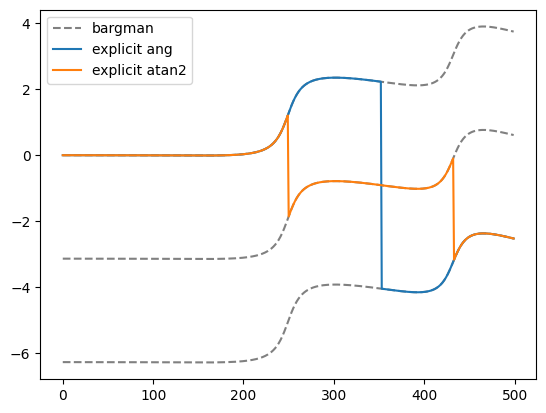
\includegraphics[width = 0.6\textwidth]{fig/premier_resultat}
	\caption[Evolution de la phase géométrique d'un signal AM-FM-PM]{Evolution de la phase géométrique d'un signal AM-FM-PM généré. En gris la phase géométrique du signal calculé via l'invariant de Bargmann. Les deux autres sont calculées avec la formule \cref{eq:phaseg_2var}, en bleu en utilisant de l'argument pour la phase totale et en orange en utilisant atan2.}
\end{figure}

Deux remarques sur ces formules. 
La première est que la phase géométrique ne dépend que des paramètres de polarisations $\theta$ et $\chi$, ce qui reflète son invariance par transformation de jauge.
La seconde, nettement plus troublante, est que $\varphi$ ne s'interprète ni comme phase totale ni comme phase dynamique. 
%Plus loin, \thoughts{\cref{subsec:aller_plus_loin}}, nous reviendrons sur laquelle des deux ``doit'' représenter $\varphi$.
\\
Pour que ce soit le cas, il faut qu'à l'instant $t$, $\x $ retrouve la même polarisation instantanée qu'à l'instant $t_0$, auquel cas :
\begin{equation}\label{eq:phases_p-cyc_2var}
	\begin{aligned}
		\big( \chi(t), \theta(t) \big) = \big( \chi(t_0), \theta(t_0) \big)\quad 
		&\Lr\quad \phaset(\x ) = \varphi(t) - \varphi(t) \\
		&\Lr\quad \phaseg(\x ) = -\int_{t_0}^t \theta'(s) \sin 2\chi(s) ds
	\end{aligned}
\end{equation}
\skipl

Même dans ce cas, il est utile de d'avoir une représentation de $\x $ qui soit indépendante de sa phase pour interpréter cette formule \eqref{eq:phases_p-cyc_2var}.
\\



\subsection{Interprétation sur la sphère de Poincaré}\label{subsec:phase_g2Poincare}

Dans l'étude de la phase géométrique, il est standard de s'intéresser à la matrice de covariance\footnote{\itshape
	La conjugaison ici est à gauche pour simplifier l'interprétation de $\rho$ dans la \Cref{fig:sphere2poincare}
} :
\begin{equation} \label{eq:proj2x_2var}
	\forall t\in\R,\quad \rho_{\x}(t) = \frac{1}{\|\x(t) \|^2} \congu{\x(t) }\, ^t\x(t)
\end{equation}
\\
Outre son utilité en traitement du signal, elle présente l'avantage d'être invariante par transformation de de jauge (\ie~ $\rho_{e^{i\alpha}\x} = \rho_{\x}$).
Dans le cas des AM-FM-PM, Le Bihan \etal~ont montré qu'elle se décompose dans la base de Pauli comme :
\begin{equation} \label{eq:decompo_pauli}
	\rho_{\x} = \frac{1}{2}\Big( id + \sin(2\theta) \cos(2\chi) \sigma_1 + \sin (2\chi) \sigma_2 + \cos(2\theta) \cos(2\chi) \sigma_3 \Big)
\end{equation}


\begin{wrapfigure}{r}{0.4\textwidth}
	\begin{tikzpicture}[scale=0.8]
	%\draw[black, opacity=0.1] (-4.5,-4.5) grid (4.5,4.5);
	\draw[-Stealth] (-2.5,0) -- (4.5,0) node[below]{$\sigma_1$};
	\draw[-Stealth] (0,-4.5) -- (0,4.5) node[right]{$\sigma_2$};
	\draw[-Stealth] (2.5,1.2) -- (-2.5,-1.2)  node[below right]{$\sigma_3$};
	
	\coordinate (o) at (0,0);
	\coordinate (i) at (4,0);
	\coordinate (j) at (0,4);
	
	\coordinate (u) at (2.1,2.14);
	\coordinate (p) at (2.1, -0.5);
	\coordinate (v) at (3.4,0.5);
	
	% cercles
	\draw[thick] (4,0) arc [start angle=0, end angle =-140, radius = 4];
	\draw[thick] (4,0) arc [start angle=0, end angle =100, radius = 4];
	
	\draw[thick, dashed] (4,0) arc [start angle=0, end angle =100, radius = 4, y radius = 1];
	\draw[thick] (4,0) arc [start angle=0, end angle =-125, x radius = 4, y radius = 1];
	
	% droites
	\draw[-stealth,thick, blue] (0,0) -- (u) node[above right] {$\rho$};
	\draw[dashed, blue] (u) -- (p);
	\draw[dashed, blue] (0,0) -- (p);
	
	%arc au point
	\draw[gray, dashed] (3.1,2.5) arc [start angle=0, end angle =105, radius = 3.1, y radius = 0.5];
	\draw[gray] (3.1,2.5) arc [start angle=0, end angle =-120, x radius = 3.1, y radius = 0.5];
	
	\draw[violet, -stealth] (-0.4, -0.2) arc [start angle=-120, end angle =-40, x radius = 0.9, y radius = 0.225] node[midway, below] {\scriptsize$2\theta$};    
	\draw[violet, -stealth] (0,0.7) arc [start angle=90, end angle =20, x radius = 0.4, y radius = 0.5];
	\draw[violet] (0.25, 0.8) node{\scriptsize$2\chi$};
\end{tikzpicture}
	\caption{Sphère de Poincaré, \thoughts{REVOIR LES AXES ET ANGLES}}
	\label{fig:sphere2poincare}
\end{wrapfigure}

\par \noindent
où les $\sigma_i$ s'écrivent :
\begin{align*}
	\sigma_1 &= \begin{pmatrix} 0 & 1 \\ 1 &  0 \end{pmatrix}  &
	\sigma_2 &= \begin{pmatrix} 0 & -i \\  i &  0 \end{pmatrix}  &
	\sigma_3 &= \begin{pmatrix} 1 & 0 \\ 0 & -1 \end{pmatrix}
\end{align*}
\skipl

Dans cette décomposition, la composante en $id$ est indépendante de $\x$ et peut donc être ignorée (idem pour le facteur $\nicefrac{1}{2}$). Cela ne laisse qu'un vecteur (normé) de dimension 3 dont $2\theta$ et $2\chi$ correspondent aux coordonnées polaire conformément à la \Cref{fig:sphere2poincare} ci-contre.
\\ 
\\
La sphère alors obtenue, plus connue sous le nom de sphère de Poincaré, représente l'ensemble des états de polarisation possibles pour un signal :
\\
À l'équateur, la polarisation est linéaire et $\theta$ pilote son orientation et plus $\rho_{\x}$ se rapproche des pôles, plus cette polarisation devient elliptique, jusqu'à devenir complètement circulaire, auquel cas $\theta$ devient insignifiant. 
Aussi, suivant le schéma \cref{fig:ellipse2polat}, l'hémisphère nord (resp. sud) correspond à des polarisations elliptiques anti-horaire (resp. horaire).

Le fait que ce soit deux fois les angles qui sont représentés tient naturellement compte des potentielles redondances dans les $(\theta,\chi)$. 
Par exemple si $\x$ à pour paramètre de polarisation instantanée $(\theta_0, \chi_0)$, alors par symétrie de l'ellipse, $(\theta_0+\pi, \chi_0)$ est aussi une représentation valide. Autre exemple, si $\chi_0 = \nicefrac{\pi}{4}$, alors la polarisation est circulaire et indépendant de $\theta_0$.
\\
Dans les deux cas, la représentation dans la sphère de Poincaré évite ces problèmes puisque, dans le premier cas $(2\theta_0, 2\chi_0)$ et $(2\theta_0+2\pi, 2\chi_0)$ représente le même point, et dans le second, le point associé à $2\chi_0=\nicefrac{\pi}{2}$ (pôle nord) est indépendant du choix de $\theta_0$.
\\

\begin{figure}[h]
	
\includegraphics[width=0.8\textwidth]{fig/placeholder}
	\caption{Représentation des paramètres de polarisation instantanée associés à chaque point de la sphère de Poincaré.}
\end{figure}


Pour interpréter la formule \eqref{eq:phases_p-cyc_2var} de la phase géométrique prenons un exemple. Si $\chi$ et $\theta$ sont telle que :
\begin{align*}
	\theta(t_0) &= 0  &  \theta(t) &= 2\pi  &  \chi(s) &= \chi_0
\end{align*}
\\
Alors $\rho_{\x}$ décrit un chemin horizontal sur la sphère, $\rho_{\x}(t_0) = \rho_{\x}(t)$ et sa phase géométrique s'écrit\footnote{\itshape 
	L'on retrouve dans cette formule le fait que $\phaseg$ est indépendant de la paramétrisation : le résultat est indépendant des l'évolution de $\theta$ sur $]t_0,t[$.} :
\begin{align*}
	\phaseg(\x, t_0, t) = -\int_{t_0}^t \theta'(s) \sin 2\chi(s) ds &= - \sin 2\chi_0 \int_{t_0}^t \theta'(s) ds \\
	&= - \sin 2\chi_0 \big( \theta(t) - \theta(t_0)\big) \\
	&= - 2\pi\sin 2\chi_0
\end{align*}
\skipl

Formule qui est égale, à $2\pi$ près, à d'aire de la calotte entourée par $\rho_{\x}$, à savoir :
\[\mathcal{A}ire(\chi_0) = 2\pi - 2\pi \sin(2\chi_0)\]
\\
Pour être précis, pour tenir compte du fait que $\x$ ait fait une rotation complète, il est plus naturel de prendre comme phase totale :
\[\phaset(\x) = \varphi(t) - \varphi(t_0) + 2\pi\]
\\
Auquel cas, la phase géométrique donne exactement l'aire de la calotte. Dans la même logique, si l'état de polarisation subit une rotation de $n$ tours, alors $\theta$ va de $0$ à $2n\pi$ et :
\[\phaseg(\x) = 2n\pi - 2n\pi\sin(2\chi_0) = n\mathcal{A}ire(\chi_0)\]
\\
Ainsi, même si $\phaseg$ est définie modulo $2\pi$, le choix du représentant reste important pour mieux tenir compte de l'évolution de $\rho_{\x}$ au court du temps.
\\

En revanche, l'aire totale de la sphère est de $4\pi$, donc l'aire de toute surface de $S^2$ peut être vue comme étant définie modulo $4\pi$, ce qui n'est pas cohérent avec la phase géométrique, qui elle l'est à $2\pi$ près.
\\
Pour résoudre ce problème apparent, il suffit de noter que, tant dit que l’ellipse de polarisation de $\x$ à fait un tour complet, 
$\rho_{\x}$ en a effectué deux sur la sphère ($2\theta(t) = 4\pi$).
Pour qu'il n'en fasse qu'un, il faut faire varier $\theta$ de 0 à $\pi$, auquel cas le terme de la phase géométrique hérité de la $\phaset$ vaut $\pi$ et :
\begin{equation} \label{eq:phase_g2calotte}
	\phaseg(\x, t_0, t) = \pi - \pi\sin 2\chi_0 = \frac{1}{2}\mathcal{A}ire(\chi_0)
\end{equation}
\\
Dans ce cas, la phase géométrique s'interprète comme la demi-aire de la surface entourée par $\rho_{\x}$. Cela n'est, pour l'instant, valable que pour le cas particulier où $\chi$ est constant mais il sera montré dans la \cref{part:phase_geo} que cela se généralise très bien.
\\

Cela étant dit, le fait que $\rho_{\x}$ doive faire deux tours pour que $(\theta,\chi)$ retourne à son état initiale, met en évidence un problème quand à la paramétrisations de l'ellipse de polarisation.
\\
Toujours à $\chi$ fixé, si $\theta$ se voit ajouter $\pi$, alors l'état de polarisation est le même , comme expliqué plutôt : $\ \rho(\theta+\pi,\chi) = \rho(\theta, \chi)$.
En revanche, si l'on s'intéresse à un point particulier de l'ellipse, après une rotation de $\pi$, ce même point se retrouvera à l'opposé de là où il était auparavant. 
En d'autre termes, il a subi une rotation de $\pi$ mais qui apparaît non plus dans l'état de polarisation $\rho_{\x}$ mais dans la phase totale (\cref{eq:phase_g2calotte}).
\\
Sachant que $S^2$ est une représentation de rotation $\SO(3)$ de $\R^3$, ce lien entre l'évolution de $\x$ est le nombre de rotations de $\rho_{\x}$ sur $S^2$, n'est pas sans rappeler le fait que $\SU(2)$ soit connu pour être un double recouvrement de ce dernier.
\\




\subsection{\todo Généralisation en plus haute dimension} \label{subsec:aller_plus_loin}

\begin{itemize}
	
	\item Différentes écritures du bivarié pour différentes généralisation :
	
	\item Les quaterions on passe vites parce que ca se généralise très mal, Lefevre a a parlée, ca mène aux algèbres Clifford : trop de contrainte sur les dimensions des signaux
	
	\item En terme d'expo de matrice ? Lefevre \cite[sec. I.3]{lefevre_polarization_2021} l'a fait en trivarié mais au delà, y'a plus vraiment de choix remarquable de base pour $\mathfrak{u}(n)$
	
	\item En augmentant la taille de la matrice de rotation ? Lilly \cite{lilly_modulated_2011} l'a fait en trivarié et mais là encore, en terme de généralisation c'est pas si dingue parce que la matrice de rotation est pas calculable.
	
	\item Dans tout ça, on ratte le plus important : La phase géo est invariante par transfo de jauge, donc il faut faut faire apparaître $\PC{n-1}$ dans la décomposition.
	
	\item et en fait, c'est le cas en bivarié car $\PC{1}\cong \S{2}$ !
	
	\item $\PC{n-1}$ oui mais il faut pas non plus regarder que la projection parce qu'on perd toute les phases dans ce cas.
	
	\item Le bon compromis c'est les variétés fibrées : on est dans $\PC{n-1}$ mais on garde les phases dans les fibres.
	
	\item D'autant plus que ça à déjà était fait en physique et c'est vraiment concluant... (transition vers la grande partie suivante.)
	
\end{itemize}

Au niveau des ensembles, décomposer un signal multivarié complexe en paramètre d'amplitude, phase et polarization instantanée, revient à décomposer $\C^n$ en un produit de trois ensembles. Pour cela, un vecteur de $\C^n$ est vu comme la donné d'une direction, \ie~un élément de la sphère unité $S^{2n-1}\subset\C^n$, et d'une norme, de sorte que :
\[\C^n \cong \R^{+_*} \times S^{2n-1}\]
\\
Les éléments de $\R^{+_*}$ s'interprète naturellement comme l'amplitude instantanée du signal et pour faire apparaître sa phase, $S^{2n-1}$ est lui-même décomposé de sorte à faire apparaître $\U{1}$, donnant :
\[\C^n \cong \R^{+_*} \times \U{1} \times S^{2n-1}/\U{1}\]
Le quotient restant n'est autre que l'espace projectif complexe de dimension (complexe) $n-1$, noté $\PC{n-1}$. Sa construction sera détaillée dans la \cref{part:phase_geo} suivante.
\\

Pour motiver d'autant plus cette décomposition, la projection $\rho : \x \lr \congu{\x}\,^t\x / \|\x\|^2$, qui s'est avérée fort instructive, peut être vue comme une projection sur l'espace complexe en cela qu'elles sont toutes deux invariantes par transformation de jauge\footnote{\itshape
	Pour être précis, c'est le premier théorème d'isomorphisme assure $\rho(\C^n) \cong\PC{n-1}$ sont en bijection et de même structure.}.
En particulier, si $n=2$, $\PC{1}\cong S^{2}$, soit exactement l'espace de représentation des $\rho_{\x}$ dans la section précédente.
